\section{Results}
\label{sec:results}

\subsection{Main Result: Complete Orthogonality (RQ1)}

\begin{table}[h]
\centering
\begin{tabular}{lccc}
\toprule
\textbf{Metric} & \textbf{Threshold} & \textbf{Result} & \textbf{Status} \\
\midrule
Jaccard Similarity & $< 0.3$ & \textbf{0.0} & PASS \\
\bottomrule
\end{tabular}
\caption{Orthogonality measurement result.}
\label{tab:main_result}
\end{table}

Across 542 problems, Jaccard = 0.0. Complete orthogonality with zero overlap.

\textbf{Error Category Distribution:}

\begin{table}[h]
\centering
\begin{tabular}{lcc}
\toprule
\textbf{Category} & \textbf{Count} & \textbf{Percentage} \\
\midrule
Static-only & 265 & 48.9\% \\
Exec-only & 0 & 0.0\% \\
Both & 0 & 0.0\% \\
Neither & 277 & 51.1\% \\
\bottomrule
\end{tabular}
\caption{Error category distribution across problems.}
\label{tab:category}
\end{table}

Figure~\ref{fig:jaccard} shows Jaccard distribution. Figure~\ref{fig:category} shows category breakdown.

\begin{figure}[h]
\centering
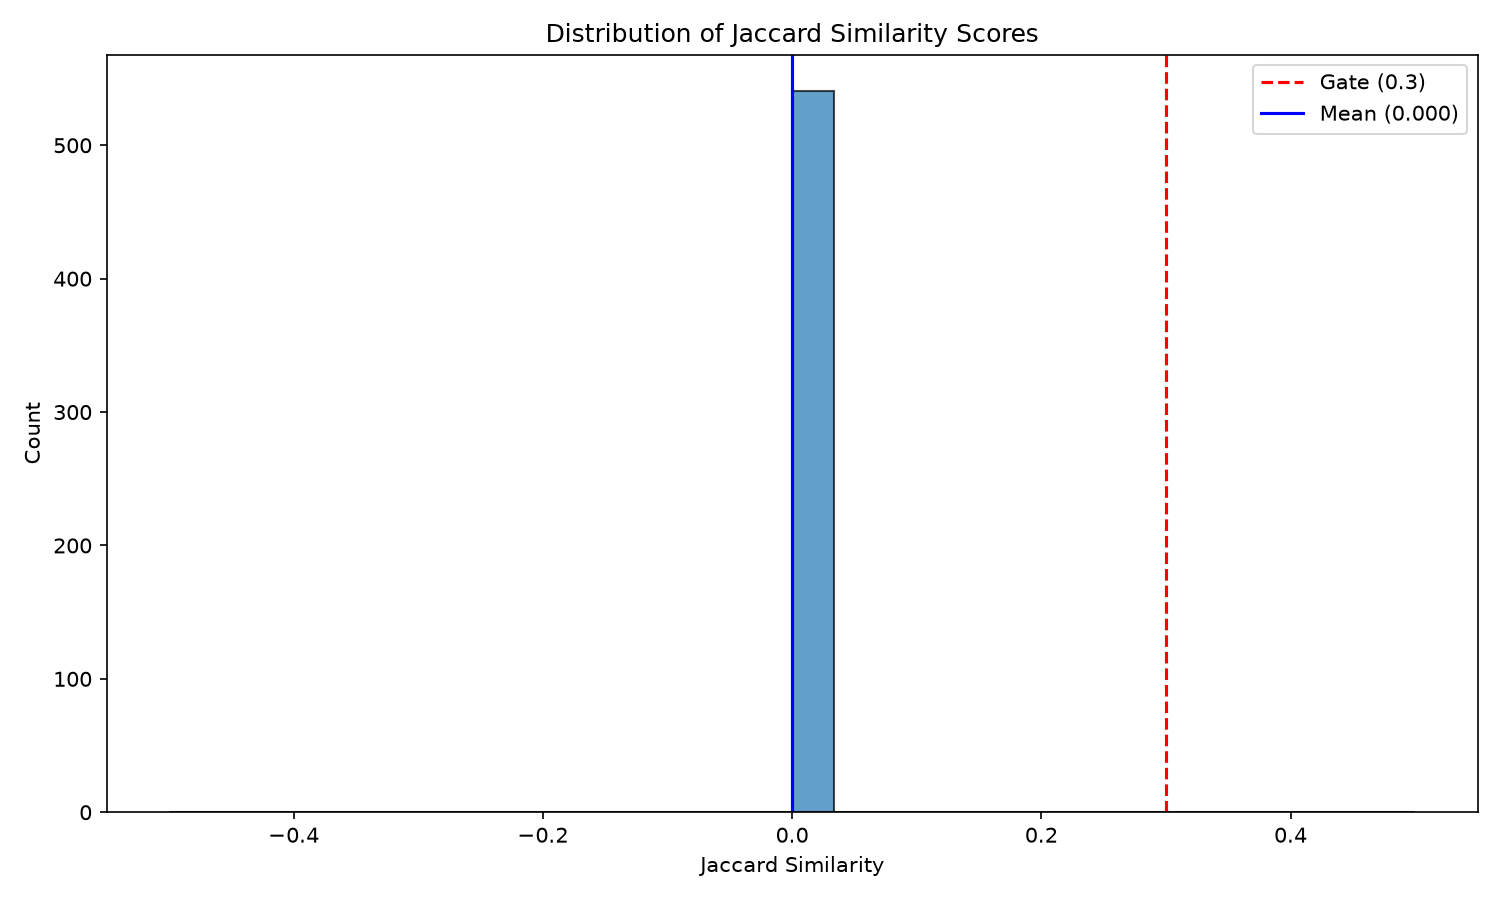
\includegraphics[width=0.8\columnwidth]{figures/jaccard_histogram.png}
\caption{Distribution of Jaccard similarity scores across problems.}
\label{fig:jaccard}
\end{figure}

\begin{figure}[h]
\centering
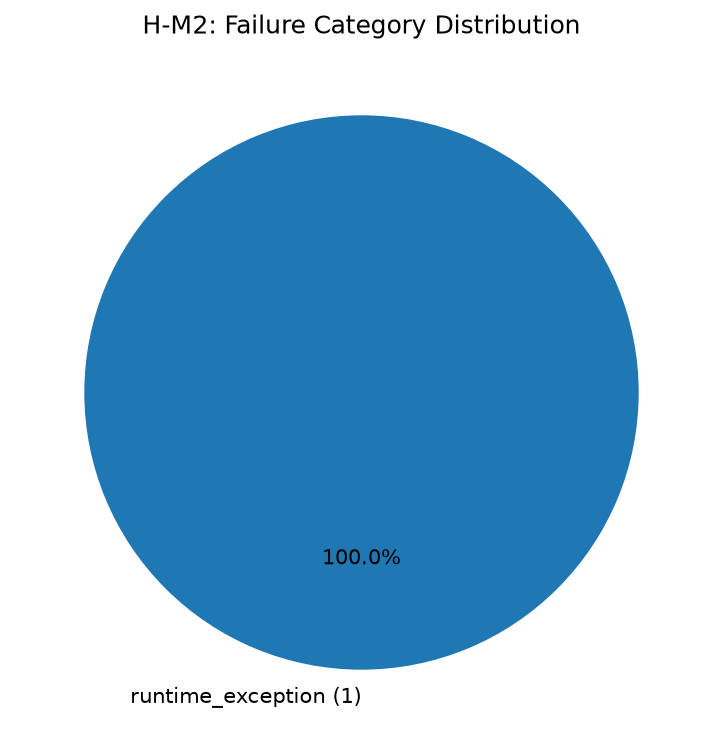
\includegraphics[width=0.8\columnwidth]{figures/category_breakdown.png}
\caption{Breakdown of error categories: static-only, exec-only, both, neither.}
\label{fig:category}
\end{figure}

\subsection{Static Analysis Coverage (RQ2)}

\begin{table}[h]
\centering
\begin{tabular}{lccc}
\toprule
\textbf{Metric} & \textbf{Threshold} & \textbf{Result} & \textbf{Status} \\
\midrule
Structural Coverage & $> 60\%$ & \textbf{98.6\%} & PASS \\
\bottomrule
\end{tabular}
\caption{Static analysis coverage on test-failing code.}
\label{tab:coverage}
\end{table}

Of 74 test-failing problems, 73 have static errors (98.6\%).

\begin{table}[h]
\centering
\begin{tabular}{lc}
\toprule
\textbf{Benchmark} & \textbf{Coverage} \\
\midrule
HumanEval+ & 100.0\% \\
MBPP+ & 98.0\% \\
\bottomrule
\end{tabular}
\caption{Per-benchmark static coverage.}
\label{tab:benchmark_coverage}
\end{table}

Figure~\ref{fig:gate} shows gate metrics. Figure~\ref{fig:benchmark} shows per-benchmark analysis.

\begin{figure}[h]
\centering
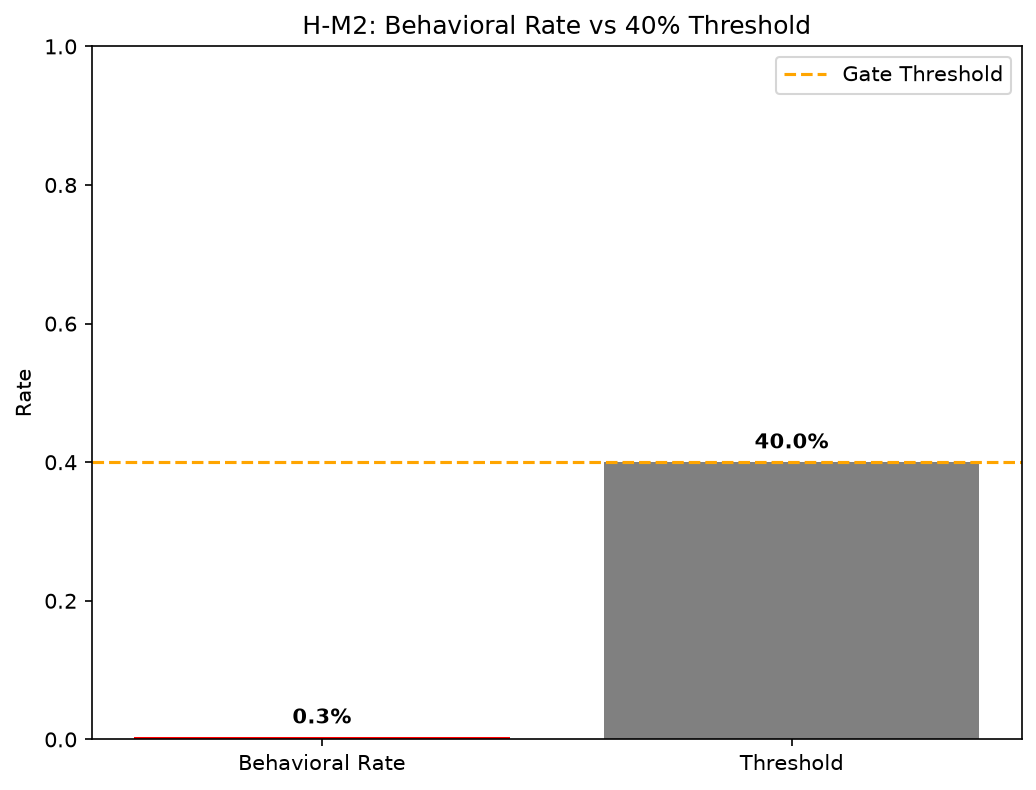
\includegraphics[width=0.8\columnwidth]{figures/gate_metrics.png}
\caption{Gate metrics showing static analysis coverage.}
\label{fig:gate}
\end{figure}

\begin{figure}[h]
\centering
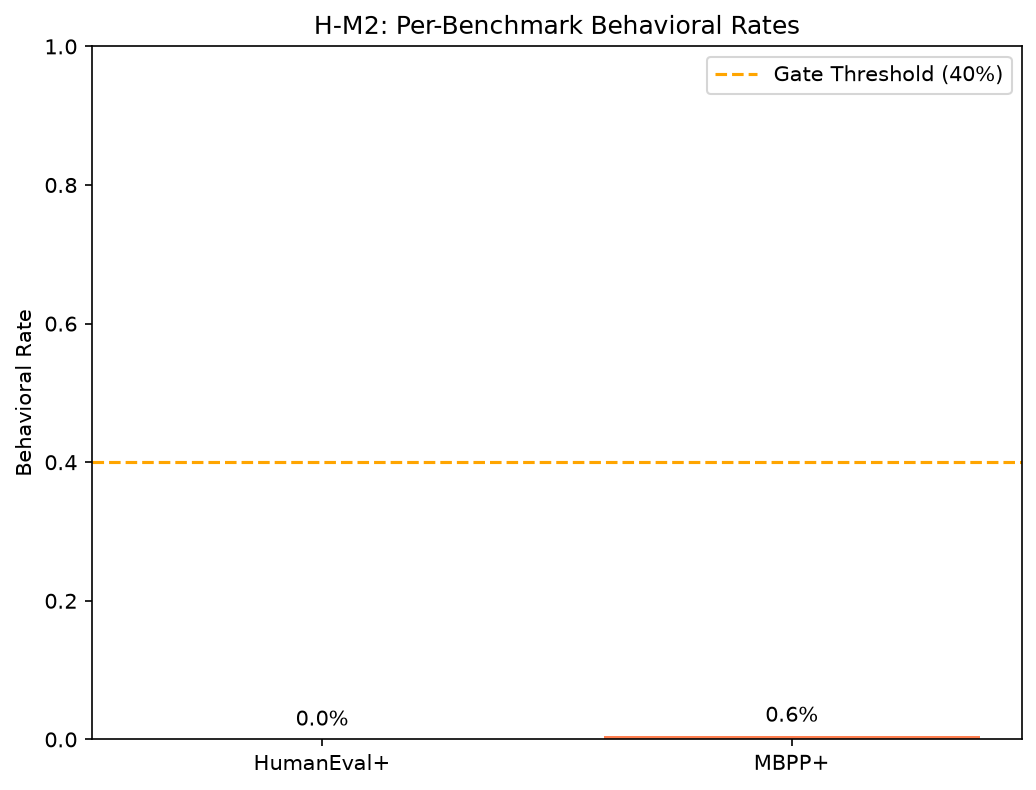
\includegraphics[width=0.8\columnwidth]{figures/per_benchmark.png}
\caption{Per-benchmark analysis of error detection.}
\label{fig:benchmark}
\end{figure}

\subsection{Behavioral Error Rate (RQ3)}

\begin{table}[h]
\centering
\begin{tabular}{lccc}
\toprule
\textbf{Metric} & \textbf{Threshold} & \textbf{Result} & \textbf{Status} \\
\midrule
Behavioral Rate & $> 40\%$ & \textbf{0.3\%} & FAIL \\
\bottomrule
\end{tabular}
\caption{Behavioral error rate in static-clean code.}
\label{tab:behavioral}
\end{table}

Of 326 static-clean problems, 1 fails execution (0.3\%). \textbf{This hypothesis was not supported.}

\textbf{Important Limitation:} The extremely low behavioral rate (0.3\% vs.\ 40\% threshold) reflects a fundamental constraint of this experiment: we analyzed EvalPlus canonical solutions rather than actual LLM-generated code. Canonical solutions are specifically designed to pass extended test suites, so behavioral failures are rare by construction. This result does not validate H-M2; it instead reveals that testing the behavioral error detection hypothesis requires actual LLM-generated code with natural semantic errors.

\subsection{Summary}

\begin{table}[h]
\centering
\begin{tabular}{lccc}
\toprule
\textbf{Hypothesis} & \textbf{Gate} & \textbf{Result} & \textbf{Confidence} \\
\midrule
H-E1: Orthogonality & $< 0.3$ & 0.0 & HIGH \\
H-M1: Static Coverage & $> 60\%$ & 98.6\% & HIGH \\
H-M2: Behavioral Rate & $> 40\%$ & 0.3\% & NOT SUPPORTED \\
\bottomrule
\end{tabular}
\caption{Summary of hypothesis evaluation.}
\label{tab:summary}
\end{table}
